\documentclass{article}
\usepackage{amsmath}
\usepackage{tikz}
\begin{document}

\begin{figure}[htbp]
\centering
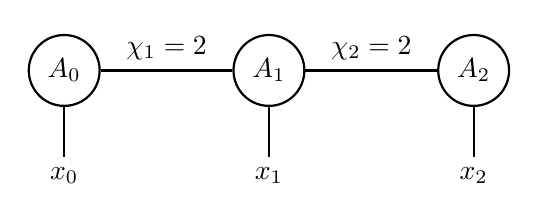
\begin{tikzpicture}[core/.style={circle, draw, thick, minimum size=9mm}, bond/.style={thick}, leg/.style={thick}]
  \node[core] (A0) at (0.00, 0) {$A_{0}$};
  \draw[leg] (A0) -- (0.00, -1.1) node[below] {$x_{0}$};
  \node[core] (A1) at (2.60, 0) {$A_{1}$};
  \draw[leg] (A1) -- (2.60, -1.1) node[below] {$x_{1}$};
  \node[core] (A2) at (5.20, 0) {$A_{2}$};
  \draw[leg] (A2) -- (5.20, -1.1) node[below] {$x_{2}$};
  \draw[bond] (A0) -- node[above] {$\chi_{1}=2$} (A1);
  \draw[bond] (A1) -- node[above] {$\chi_{2}=2$} (A2);
\end{tikzpicture}

\medskip
\begin{minipage}{\linewidth}
\begin{align*}
A_{0}^{(0)} &= \begin{pmatrix}-0.27 & 0.36\end{pmatrix} \\
A_{0}^{(1)} &= \begin{pmatrix}0.89 & 0.11\end{pmatrix} \\
A_{1}^{(0)} &= \begin{pmatrix}-0.65 & -0.10 \\ -0.49 & 0.81\end{pmatrix} \\
A_{1}^{(1)} &= \begin{pmatrix}-0.75 & 0 \\ 0.32 & 0\end{pmatrix} \\
A_{2}^{(0)} &= \begin{pmatrix}0 \\ 1\end{pmatrix} \\
A_{2}^{(1)} &= \begin{pmatrix}-1 \\ 0\end{pmatrix}
\end{align*}
\end{minipage}
\caption{Right-canonical tensor train of the state of Fig.~1(a) in Hillmich et al.: $\psi(x_0 x_1 x_2) = A_0^{(x_0)} A_1^{(x_1)} A_2^{(x_2)}$.}
\end{figure}

\begin{figure}[htbp]
\centering
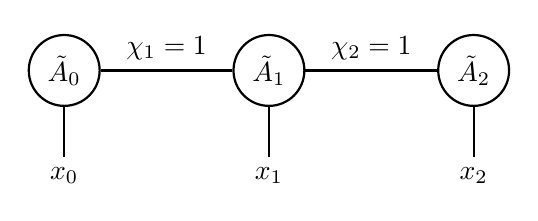
\begin{tikzpicture}[core/.style={circle, draw, thick, minimum size=9mm}, bond/.style={thick}, leg/.style={thick}]
  \node[core] (A0) at (0.00, 0) {$\tilde A_{0}$};
  \draw[leg] (A0) -- (0.00, -1.1) node[below] {$x_{0}$};
  \node[core] (A1) at (2.60, 0) {$\tilde A_{1}$};
  \draw[leg] (A1) -- (2.60, -1.1) node[below] {$x_{1}$};
  \node[core] (A2) at (5.20, 0) {$\tilde A_{2}$};
  \draw[leg] (A2) -- (5.20, -1.1) node[below] {$x_{2}$};
  \draw[bond] (A0) -- node[above] {$\chi_{1}=1$} (A1);
  \draw[bond] (A1) -- node[above] {$\chi_{2}=1$} (A2);
\end{tikzpicture}

\medskip
\begin{minipage}{\linewidth}
\begin{align*}
\tilde A_{0}^{(0)} &= \begin{pmatrix}0.26\end{pmatrix} \\
\tilde A_{0}^{(1)} &= \begin{pmatrix}-0.97\end{pmatrix} \\
\tilde A_{1}^{(0)} &= \begin{pmatrix}-0.66\end{pmatrix} \\
\tilde A_{1}^{(1)} &= \begin{pmatrix}-0.75\end{pmatrix} \\
\tilde A_{2}^{(0)} &= \begin{pmatrix}0\end{pmatrix} \\
\tilde A_{2}^{(1)} &= \begin{pmatrix}1\end{pmatrix}
\end{align*}
\end{minipage}
\caption{The same tensor train truncated to $\chi=1$: fidelity $F=0.853$ with the exact state.}
\end{figure}

\end{document}
